\documentclass{article}
\usepackage{amsfonts, amsthm, amsmath, amssymb, mathtools, ulem, mathrsfs, physics, esint, siunitx, tikz-cd}
\usepackage{pdfpages, fullpage, color, microtype, cancel, textcomp, markdown, hyperref, graphicx}
\usepackage{enumitem}
\graphicspath{{./images/}}
\usepackage[english]{babel}
\usepackage[autostyle, english=american]{csquotes}
\MakeOuterQuote{"}
\usepackage{xparse}
\usepackage{tikz}
\usepackage{algpseudocode}

% fonts
\def\mbb#1{\mathbb{#1}}
\def\mfk#1{\mathfrak{#1}}
\def\mbf#1{\mathbf{#1}}
\def\tbf#1{\textbf{#1}}

% common bold letters
\def\bP{\mbb{P}}
\def\bC{\mbb{C}}
\def\bH{\mbb{H}}
\def\bI{\mbb{I}}
\def\bR{\mbb{R}}
\def\bQ{\mbb{Q}}
\def\bZ{\mbb{Z}}
\def\bN{\mbb{N}}

% brackets
\newcommand{\br}[1]{\left(#1\right)}
\newcommand{\sbr}[1]{\left[#1\right]}
\newcommand{\brc}[1]{\left\{#1\right\}}
\newcommand{\lbr}[1]{\left\langle#1\right\rangle}

% matrices
\newcommand{\m}[2][b]{\begin{#1matrix}#2\end{#1matrix}}
\newcommand{\arr}[3][\sbr]{#1{\begin{array}{#2}#3\end{array}}}

% misc
\NewDocumentCommand{\app}{O{x} O{\infty}}{\xrightarrow{#1\to#2}}
\renewcommand{\ss}{\subset}
\newcommand{\vn}{\varnothing}
\newcommand{\inv}{^{-1}}
\newcommand{\imp}{\implies}
\newcommand{\impleft}{\reflectbox{$\implies$}}
\renewcommand{\bar}{\overline}
\renewcommand{\d}{\partial}
\newcommand{\pf}{\tbf{Proof. }}

% greek
\newcommand{\e}{\epsilon}
\newcommand{\p}{\varphi}
\renewcommand{\t}{\theta}
\renewcommand{\a}{\alpha}
\renewcommand{\b}{\beta}

% title
\title{Scientific Computing HW 8}
\author{Ryan Chen}
%\date{\today}
\setlength{\parindent}{0pt}


\begin{document}
	
\maketitle



\begin{enumerate}
	
	
	
	\item To show that the algorithms are equivalent, we rewrite $\a_k,r_{k+1},\b_{k+1}$. Rewrite $\a_k$ as
	\begin{align*}
		\a_k &= -\frac{r_k^Tp_k}{p_k^TAp_k} \\
		&= -\frac{r_k^T(-r_k+\b_kp_{k-1})}{p_k^TAp_k} & p_k = -r_k+\b_kp_{k-1} \\
		&= \frac{r_k^Tr_k}{p_k^TAp_k} & \text{$r_k^Tp_{k-1}=0$ by Theorem 5.2 in [NW]}
	\end{align*}
	Rewrite $r_{k+1}$ as
	\begin{align*}
		r_{k+1} &= Ax_{k+1} - b \\
		&= A(x_k+\a_kp_k) - b \\
		&= Ax_k - b + \a_kAp_k \\
		&= r_k + \a_kAp_k
	\end{align*}
	The expressions for $\a_k,r_{k+1}$ give
	\[Ap_k = \frac{r_{k+1}-r_k}{\a_k} = \frac{p_k^TAp_k(r_{k+1}-r_k)}{r_k^Tr_k}\]
	Use this to rewrite $\b_{k+1}$ as
	\begin{align*}
		\b_{k+1} &= \frac{r_{k+1}^TAp_k}{p_k^TAp_k} \\
		&= \frac{r_{k+1}^T(r_{k+1}-r_k)}{r_k^Tr_k} \\
		&= \frac{r_{k+1}^Tr_{k+1}}{r_k^Tr_k} & \text{$r_{k+1}^Tr_k=0$ by Theorem 5.3 in [NW]}
	\end{align*}
	
	
	
	\pagebreak
	
	
	
	\item f
	
	
	
	\pagebreak
	
	
	
	\item
	
	\begin{enumerate}
		
		
		
		\item 
		
		
		
		\item
		
		
		
		\item
		
		
		
		\item
		
		
		
		\item
		
		
		
		\item
		
		
		
	\end{enumerate}



	\pagebreak
	
	
	
	\item Code: \url{https://github.com/RokettoJanpu/scientific-computing-1-redux/blob/main/hw8/hw8.ipynb}
	
	\begin{center}
		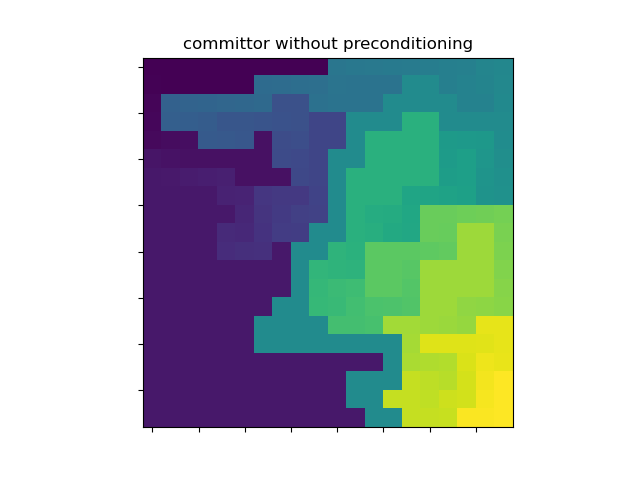
\includegraphics[scale=.4]{committor without preconditioning}
		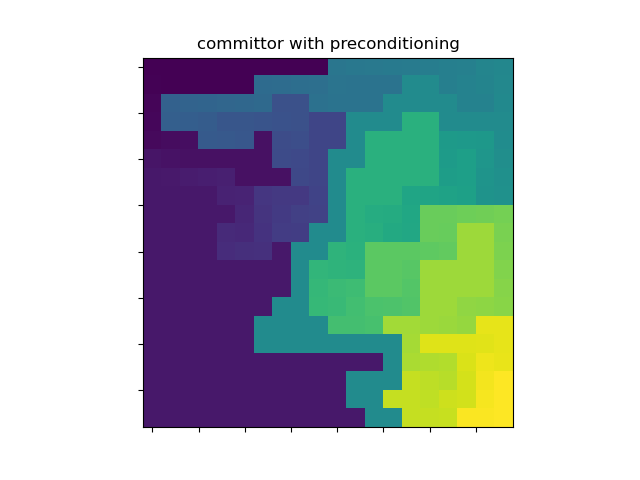
\includegraphics[scale=.4]{committor with preconditioning}
		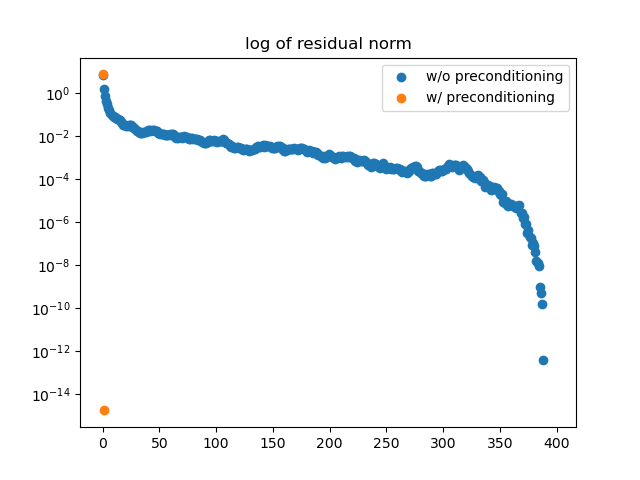
\includegraphics[scale=.5]{residual norm}
	\end{center}
	CG with conditioning only took one iteration, resulting in only two plotted points.
	
	
\end{enumerate}
	
	
	
	
\end{document}